\documentclass[conference]{IEEEtran}
% PRDC 2026 main-track case study, camera-ready: IEEE double-column,
% 6 pages excluding references. https://prdc-symposium.org/2026/
\usepackage{cite}
\usepackage{amsmath,amssymb,amsfonts}
\usepackage{graphicx}
\usepackage{booktabs}
\usepackage{tikz}
\usetikzlibrary{arrows.meta, positioning, calc}
\usepackage{xcolor}
\usepackage[hidelinks]{hyperref}
\usepackage{balance}

% IEEEtran selects Adobe Courier (pcr); its metrics are absent from some TeX
% installations, so fall back to Computer Modern typewriter.
\renewcommand{\ttdefault}{cmtt}

\newcommand{\sys}{ROOTS}
\newcommand{\Sys}{ROOTS}

\newcommand{\coderepo}{\footnote{The platform's services are public under
\url{https://github.com/ATT-Acelerar-e-Transformar-o-Turismo} (the wrapper
manager lives in \texttt{resource-service}); the analysis scripts, the derived
per-wrapper and per-repair event dataset, and the prompt templates are at
\url{https://github.com/dferrero17/observatory-artifact-prdc}.}}

% Break the column early if fewer than #1 lines remain.
\makeatletter
\newcommand{\needlines}[1]{\par
  \begingroup
  \dimen@=#1\baselineskip
  \vskip\z@\@plus\dimen@
  \penalty -100
  \vskip\z@\@plus-\dimen@
  \endgroup}
\makeatother

% Production metrics computed from the analyzed deployment dump.
% Auto-generated by analysis/compute_metrics.py -- do not edit.
% Source: the analyzed production dump (path redacted for double-blind review).
\newcommand{\nWrappers}{396}
\newcommand{\nCompleted}{170}
\newcommand{\pctCompleted}{42.9}
\newcommand{\nStopped}{141}
\newcommand{\pctStopped}{35.6}
\newcommand{\nErrorW}{69}
\newcommand{\pctErrorW}{17.4}
\newcommand{\nExecuting}{16}
\newcommand{\pctExecuting}{4}
\newcommand{\nXLSX}{188}
\newcommand{\nAPI}{184}
\newcommand{\nCSV}{24}
\newcommand{\pctXLSX}{47.5}
\newcommand{\pctAPI}{46.5}
\newcommand{\pctCSV}{6.1}
\newcommand{\pctCompletedXLSX}{55.3}
\newcommand{\pctCompletedAPI}{28.3}
\newcommand{\pctCompletedCSV}{58.3}
\newcommand{\nDomAmbiente}{203}
\newcommand{\nDomEconomia}{139}
\newcommand{\nDomSocio}{54}
\newcommand{\nRetried}{43}
\newcommand{\pctRetried}{10.9}
\newcommand{\retryOnce}{37}
\newcommand{\retryTwice}{5}
\newcommand{\retryThrice}{1}
\newcommand{\nRecovered}{39}
\newcommand{\pctRecovered}{90.7}
\newcommand{\nRecoveredXLSX}{26}
\newcommand{\nRecoveredAPI}{10}
\newcommand{\nRecoveredCSV}{3}
\newcommand{\nRecoveredRetryOnce}{33}
\newcommand{\nRecoveredRetryTwice}{5}
\newcommand{\nRecoveredRetryThrice}{1}
\newcommand{\nDataPoints}{164,322}
\newcommand{\nDataPointsXLSX}{53,530}
\newcommand{\nDataPointsAPI}{79,411}
\newcommand{\nDataPointsCSV}{31,381}
\newcommand{\medianPointsPerWrapper}{27.5}
\newcommand{\pNinetyPointsPerWrapper}{967}
\newcommand{\nZeroPointWrappers}{112}
\newcommand{\nNonzeroPointWrappers}{284}
\newcommand{\genLatencyMedian}{26.8}
\newcommand{\genLatencyPninety}{109.8}
\newcommand{\genLatencyMin}{12.3}
\newcommand{\genLatencyMax}{8,461,607}
\newcommand{\nGenLatencySamples}{331}
\newcommand{\healLatencyMedian}{33.4}
\newcommand{\healLatencyPninety}{60.5}
\newcommand{\healLatencyMin}{15.5}
\newcommand{\healLatencyMax}{80.4}
\newcommand{\nHealEvents}{50}
\newcommand{\coverageMedianYears}{0.9}
\newcommand{\coverageMaxYears}{25}
\newcommand{\nCoverageWrappers}{11}
\newcommand{\coverageOldestYear}{2000}
\newcommand{\coverageNewestYear}{2026}
\newcommand{\nLowMarkSet}{11}
\newcommand{\nHighMarkSet}{279}
\newcommand{\deploymentDays}{149}
\newcommand{\deploymentStart}{January 13, 2026}
\newcommand{\deploymentEnd}{June 11, 2026}
\newcommand{\nStoppedTimeout}{15}
\newcommand{\nStoppedResourceDeleted}{126}
\newcommand{\nStoppedOther}{0}

% New PRDC analyses (analysis/prdc/ in the sibling att-etl repo). Placeholders
% until the analysis finishes; every value below is then set from its output.
\newcommand{\expMedianDays}{XX}
\newcommand{\expQone}{XX}
\newcommand{\expQthree}{XX}
\newcommand{\expMinDays}{XX}
\newcommand{\expMaxDays}{XX}
\newcommand{\expUnderDay}{XX}
\newcommand{\expOverWeek}{XX}
\newcommand{\expWrapperDays}{XX}
\newcommand{\costGenMedianUSD}{XX}
\newcommand{\costRepairMedianUSD}{XX}
\newcommand{\costTotalUSD}{XX}
\newcommand{\costInPrice}{XX}
\newcommand{\costOutPrice}{XX}
\newcommand{\costPriceDate}{XX}
\newcommand{\spotN}{XX}
\newcommand{\spotReachable}{XX}
\newcommand{\spotOverlap}{XX}
\newcommand{\spotMatch}{XX}
\newcommand{\spotMismatch}{XX}


\begin{document}

\title{Operating LLM-Generated Data Wrappers in Production:\\
A 149-Day Case Study of What Breaks in a Smart-City Intake Layer}

\author{\IEEEauthorblockN{Daniel Martins Ferreira, Sebasti\~ao Teixeira,
Henrique Teixeira, and Osvaldo Pacheco}
\IEEEauthorblockA{IEETA, LASI, University of Aveiro, Aveiro, Portugal\\
\{danielmartinsferreira, sebastiao.teixeira, henriqueft04, orp\}@ua.pt}}

\maketitle

\begin{abstract}
Every indicator a smart-city observatory shows needs a wrapper that pulls one series
from one heterogeneous source and keeps pulling it as the source drifts, and the cost
of writing and nursing those wrappers caps how many feeds an observatory sustains. We
report a \deploymentDays{}-day production case study of an intake layer that removes
the per-source code: a non-technical user registers a source through a form, and the
platform has a large language model write, run, and repair the extraction wrapper,
mapping REST APIs, spreadsheets, and CSV files to a normalized
$(\textrm{timestamp}, \textrm{value})$ series. Over \nWrappers{} wrappers and
\nDataPoints{} measurements, at least one wrapper in seven crashed with an uncaught
exception; the repair loop stopped the crash in 42 of the 43 wrappers it reached and
restored output in 32. What filled the error column was operational: 65 wrappers
(16\%) never received code because the model's free-tier quota, an overload, or our
own restarts stopped generation, an execution watchdog we had set shorter than the
feeds' polling period killed 69 API pollers, and one crash went unrepaired because the
repair call itself hit the quota. Two of four inspected repairs recovered by
swallowing an upstream error, a move our own generation prompt prescribes, so we score
recovery as resumed output and treat value correctness as open; a re-extraction of
eight public sources matched 84 of 95 stored values exactly, the rest upstream
revisions. We close with the operational rules the deployment taught us, each of
which cost us data or the means to audit it.
\end{abstract}

\begin{IEEEkeywords}
LLM-generated code, automated program repair, data ingestion, smart-city
observatory, autonomic computing, field failure study
\end{IEEEkeywords}

\section{Introduction}
\label{sec:intro}

A city run on evidence tracks many numbers that arrive in many forms: environmental
readings from sensor APIs, visitor counts from tourism boards, energy and mobility
figures from utilities and transport operators, each with its own endpoint or
spreadsheet export, field names, date format, and language. None of it
stands still: an indicator earns its place only while it stays current, so every
feed must be pulled again and again and every upstream change absorbed without
breaking the series already built. The usual way in is to write an extraction
wrapper per source and keep it alive as the source shifts. That cost, paid once to
build and indefinitely to maintain, is why mediator-style integration has never
reached past a small set of
feeds~\cite{wiederhold1992mediators,kushmerick2000wrapper,lerman2003wrapper}, and it
caps coverage: an observatory shows whichever feeds someone found time to wire and
nurse, rather than the city.

Large language models (LLMs) can now write such wrappers from a description and a
data sample, and rewrite them from a stack trace, so a domain user can register a
source through a form and have the platform generate, run, and repair the wrapper
itself. The engineering question is not whether a model can write a wrapper, which
benchmarks already answer~\cite{arora2023evaporate,huang2024autoscraper}, but what
breaks when hundreds run unattended for months, whether the failures indict the
generated code or the environment, whether repair fixes faults or hides them, and
what an operator is left holding: dependability questions with no laboratory answer.

This paper is a case study that answers them for one deployment. \Sys{} is a
smart-city observatory of tourism-sustainability indicators for a Portuguese region,
built at the University of Aveiro under the ATT agenda, whose intake layer is built
from LLM-generated wrappers. Each wrapper is an \emph{autonomic} element in the sense of
Kephart and Chess~\cite{kephart2003vision}, managed by a monitor--analyze--plan--execute
loop over shared knowledge (MAPE-K)~\cite{ibm2005blueprint,huebscher2008autonomic}
whose actuator is a model that writes code rather than a parameter tuner; the loop
organizes the exposition and names the boundary of what it can fix
(Section~\ref{sec:related} places it against prior repair work). The adaptivity is
bounded: the platform adapts to a source's format and transport within the structured tabular
family, REST/JSON APIs, spreadsheets, and delimited files, all projected onto one
univariate $(\textrm{timestamp}, \textrm{value})$ series.

The contributions are the architecture and its one narrow contract
(Section~\ref{sec:arch}) and, mainly, the empirical findings from the
\deploymentDays{}-day run. First, the \emph{binding faults are operational, not
generated-code defects}: 65 wrappers never received code because generation failed
on quota, overload, or a platform restart, 69 API pollers were killed by a watchdog
we configured shorter than their polling period, and the one crash left unrepaired
was blocked by that same quota (Section~\ref{sec:res-faults}). Second, \emph{cheap generation
decouples attempt from yield}: only \nNonzeroPointWrappers{} of \nWrappers{} wrappers
ever produced data, and most of the rest failed loudly on quota and were deleted by
their users, shifting the bottleneck from authoring to operations
(Section~\ref{sec:res-gen}). Third, \emph{crash-triggered repair can mask faults
rather than fix them}, so we score recovery as resumed output, report the exposure
time behind that score, and treat value correctness as open
(Sections~\ref{sec:res-heal}--\ref{sec:res-cases}). Section~\ref{sec:res-cost}
adds a bounded cost estimate and a re-extraction check on the reachable public
sources; the analysis script and a derived event dataset accompany the paper.\coderepo

\section{Related Work}
\label{sec:related}

The smart-tourism literature argues for destination-scale data
infrastructure~\cite{gretzel2015smart,buhalis2013smart,ec2016etis}, while field
reports find patchy uptake and getting the data in at all as the binding constraint
on sustained
monitoring~\cite{modica2018assessment,fuchs2014big,ivarsbaidal2021measuring,ivarsbaidal2023sustainable},
saying little about how intake is built.

Autonomic computing proposed self-managing components with closed control
loops~\cite{kephart2003vision}, structured as MAPE-K~\cite{ibm2005blueprint} and
cataloged by self-* property~\cite{huebscher2008autonomic}; a recent roadmap surveys
generative models as actuators in self-adaptive systems~\cite{li2024genaisas}.

Language models write runnable programs~\cite{chen2021evaluating} and repair
them~\cite{xia2023automated} through self-critique, reflection, or execution
feedback~\cite{madaan2023selfrefine,shinn2023reflexion,chen2024selfdebug}, with
inconsistent benefit~\cite{olausson2024selfrepair}; repair has run in production at
industrial scale~\cite{marginean2019sapfix,bader2019getafix} and
autonomously~\cite{bouzenia2024repairagent}. On the data side, Evaporate synthesizes
extraction code~\cite{arora2023evaporate}, AutoScraper builds reusable
scrapers~\cite{huang2024autoscraper}, agents are benchmarked on enterprise data
workflows~\cite{lei2025spider2}, prompted and fine-tuned models handle
preprocessing~\cite{narayan2022wrangle,zhang2024jellyfish}, and detecting silent
pipeline degradation is a line of work our masking finding
motivates~\cite{tu2023autovalidate}. The loop itself is not new: the repair is LLM program repair, the generation
Evaporate-style synthesis, the probing ordinary tool use. What they do not provide,
and what we contribute, is a measured population of \emph{field} faults from a live
deployment, in the tradition of field-failure studies that found operator and
configuration faults, not code, behind most outages~\cite{gray1986why,oppenheimer2003why},
and of the finding that swallowed exceptions sit behind many production
failures~\cite{yuan2014simple}.

Wrapper induction derived extraction rules from labeled
examples~\cite{kushmerick2000wrapper,crescenzi2001roadrunner,laender2002brief,ferrara2014web},
and keeping a wrapper working as its source drifts was a problem from the
start~\cite{kushmerick2000verification,lerman2003wrapper}. Extract-transform-load
(ETL) pipelines have mostly been designed by
hand~\cite{vassiliadis2002conceptual,vassiliadis2009survey}, with automation reaching
schema matching~\cite{rahm2001survey}, curation~\cite{stonebraker2013tamer}, and
wrangling~\cite{furche2016wrangling}; dataspaces~\cite{franklin2005dataspaces},
polystores~\cite{duggan2015bigdawg}, and schema-on-read lakes make data
source-agnostic for the \emph{consumer}, while we work the producer side.

\section{Architecture and the Fixed Time-Series Contract}
\label{sec:arch}

\Sys{} runs as a set of containerized services, user, knowledge-base,
data-collector, resource, and indicator (all Python and FastAPI), reached through an
nginx gateway with a React dashboard in front. Control traffic and data traffic
ride separate RabbitMQ brokers, each service keeps its own datastore, and an optional
Keycloak provider handles single sign-on. Fig.~\ref{fig:sysarch} lays out the
components and the two planes that join them: the ingestion plane, along which
wrappers read the external sources and emit points through the data broker and the
collector to the indicator store, and the REST serving plane from the gateway to the
dashboard.

\begin{figure}[t]
\centering
\resizebox{0.82\columnwidth}{!}{% Whole-system component / deployment architecture. Two planes: a REST serving
% plane through the gateway, and an asynchronous ingestion plane across two brokers.
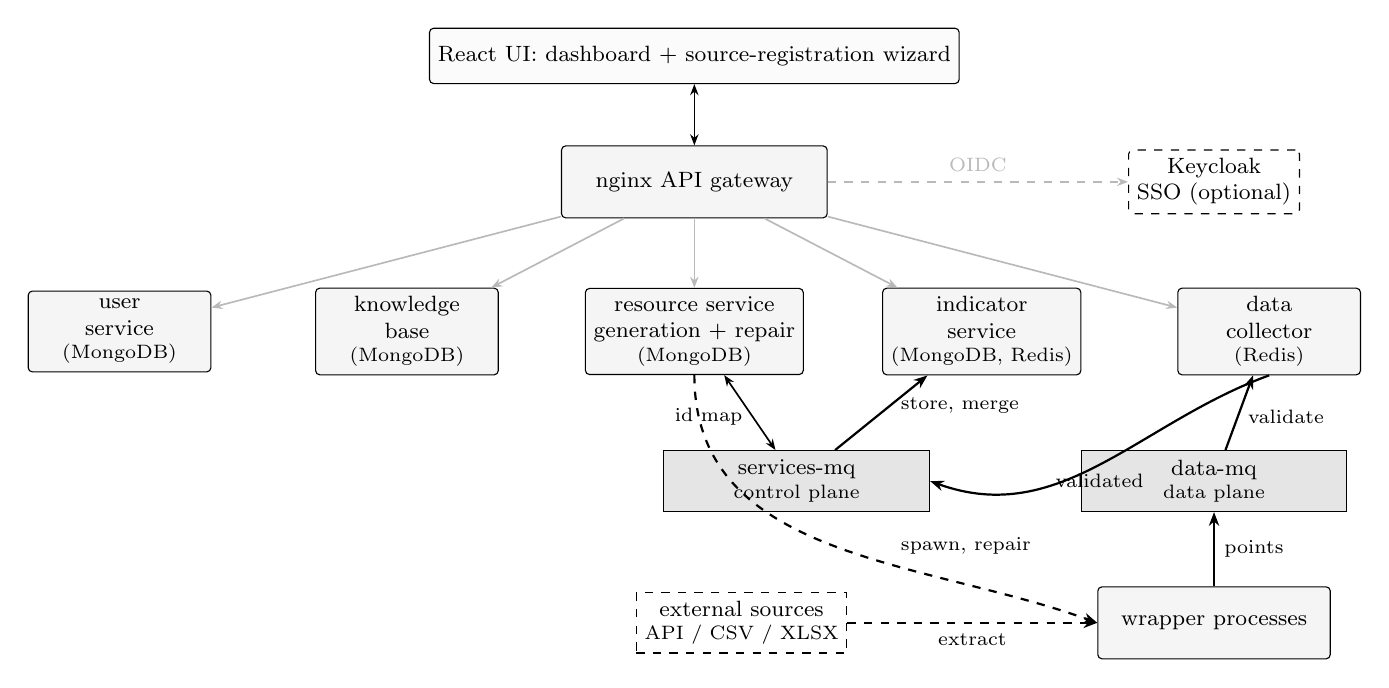
\begin{tikzpicture}[
  font=\footnotesize,
  svc/.style={draw, rounded corners=1.5pt, align=center, minimum height=26pt,
              minimum width=66pt, inner sep=3pt, fill=gray!8},
  bus/.style={draw, align=center, minimum height=22pt, minimum width=96pt,
              inner sep=3pt, fill=gray!20},
  cli/.style={draw, rounded corners=1.5pt, align=center, minimum height=20pt,
              inner sep=3pt, fill=gray!3},
  ext/.style={draw, dashed, align=center, inner sep=3pt, fill=white},
  opt/.style={draw, dashed, rounded corners=1.5pt, align=center, inner sep=3pt,
              fill=white},
  rest/.style={-{Stealth[length=4pt]}, semithick, gray!55},
  flow/.style={-{Stealth[length=5pt]}, thick},
  dep/.style={-{Stealth[length=5pt]}, thick, dashed},
  bi/.style={{Stealth[length=4pt]}-{Stealth[length=4pt]}, semithick}]

% clients, gateway, optional SSO
\node[cli] (ui) at (0,6.9) {React UI: dashboard + source-registration wizard};
\node[svc, minimum width=96pt] (gw) at (0,5.3) {nginx API gateway};
\node[opt] (kc) at (6.6,5.3) {Keycloak\\SSO (optional)};

% microservice row (Python / FastAPI), datastore noted inline
\node[svc] (us) at (-7.3,3.4) {user\\service\\[-1pt]\scriptsize(MongoDB)};
\node[svc] (kb) at (-3.65,3.4) {knowledge\\base\\[-1pt]\scriptsize(MongoDB)};
\node[svc] (rs) at (0,3.4) {resource service\\generation + repair\\[-1pt]\scriptsize(MongoDB)};
\node[svc] (is) at (3.65,3.4) {indicator\\service\\[-1pt]\scriptsize(MongoDB, Redis)};
\node[svc] (dc) at (7.3,3.4) {data\\collector\\[-1pt]\scriptsize(Redis)};

% message bus: two RabbitMQ brokers
\node[bus] (smq) at (1.3,1.5) {services-mq\\[-1pt]\scriptsize control plane};
\node[bus] (dmq) at (6.6,1.5) {data-mq\\[-1pt]\scriptsize data plane};

% ingestion workers and the external sources they read
\node[svc, minimum width=84pt] (wr) at (6.6,-0.3) {wrapper processes};
\node[ext] (src) at (0.6,-0.3) {external sources\\[-1pt]\scriptsize API / CSV / XLSX};

% --- REST serving plane (gateway fans out to every service) ---
\draw[bi] (ui) -- (gw);
\draw[rest] (gw) -- (us);
\draw[rest] (gw) -- (kb);
\draw[rest] (gw) -- (rs);
\draw[rest] (gw) -- (is);
\draw[rest] (gw) -- (dc);
\draw[rest, dashed] (gw) -- node[above, font=\scriptsize]{OIDC} (kc);

% --- asynchronous ingestion plane ---
\draw[dep] (rs.south) to[out=-90,in=160]
  node[above right, font=\scriptsize, pos=0.62]{spawn, repair} (wr.west);
\draw[flow, dashed] (src) -- node[below, font=\scriptsize]{extract} (wr);
\draw[flow] (wr) -- node[right, font=\scriptsize]{points} (dmq);
\draw[flow] (dmq) -- node[right, font=\scriptsize, pos=0.45]{validate} (dc);
\draw[flow] (dc.south) to[out=-160,in=-20]
  node[below, font=\scriptsize, pos=0.5]{validated} (smq.east);
\draw[bi] (smq) -- node[left, font=\scriptsize, pos=0.45]{id map} (rs);
\draw[flow] (smq) -- node[right, font=\scriptsize, pos=0.6]{store, merge} (is);
\end{tikzpicture}
}
\caption{Whole-system architecture. Right-hand column: the ingestion path, where
wrapper processes spawned and repaired by the resource service (dashed) read the
external sources and push points through the data-plane broker and the collector
(solid black) to the indicator store. Left: the REST serving plane, where the nginx
gateway fronts the Python/FastAPI services for the React dashboard; Keycloak provides
optional OpenID Connect (OIDC) sign-on.}
\label{fig:sysarch}
\end{figure}

Format-adaptive intake rests on one thin interface: whatever its format, a wrapper
emits point batches $\{(x,y)\}$ with $x$ an ISO~8601 timestamp and $y$ a float; the
code above that interface is generated per source, everything below it is shared
plumbing, and a source is in scope precisely when it projects onto one such series. Out of scope
by construction are unstructured content, push and streaming transports,
multivariate, geospatial, and graph data, and anything that needs a join across
feeds; the unrepairable single-column CSV of Section~\ref{sec:res-cases} is this
boundary made concrete. Four nouns recur below. A \emph{source} is the external endpoint or file; a
\emph{resource} is the platform record a user creates for it through the web wizard
(a file upload, or an API endpoint and its credentials, plus the indicator's
metadata); a \emph{wrapper} is the generated process the resource service owns for
that resource; and an \emph{indicator} is the served series the collector feeds
after validating each batch against the contract. Deleting a resource stops and
orphans its wrapper; it leaves \texttt{completed} in place but overwrites
\texttt{error} with \texttt{stopped}. Source type is
one argument to a single generation routine, not a code path of its own.

\section{One Manager per Wrapper}
\label{sec:selfstar}

Each wrapper is the element a single autonomic manager looks after: the generated
code plus its watermarks, retry counter, and status. The manager watches process
state, classifies how a process ended, plans a fresh or corrected artifact, and
deploys it, against a shared store of knowledge. Some of that knowledge is fixed: the wrapper template, which encodes the
Section~\ref{sec:arch} contract as code, and a standing list of hard rules and formatting notes distilled from earlier
failures (leave the backfill driver alone, invent no data, treat date ranges as
inclusive, never raise on an HTTP error but return an empty batch). The rest is per-wrapper and changes at runtime: a pair of watermarks (earliest
and latest timestamps sent), a retry counter capped at three, a timestamped execution
log, and the stored wrapper document (metadata, source configuration, current code,
status).

\subsection{Generation}
\label{sec:gen}
The actuator is Google's Gemini Flash, reached through the provider's Python
software development kit at default decoding settings and bound to the floating \texttt{gemini-flash-latest}
alias. It does not write code freely but fills a fixed wrapper class: only extraction
(\texttt{fetch\_external\_data}) and, for APIs, a windowed fetch and a polling period
are open to it, while the backfill driver, transport, batching, and run loop are
library code the prompt tells it not to touch. A template engine assembles the prompt from the indicator metadata, the source
configuration, a brief data sample (20 CSV lines, 15 rows per sheet, or a captured
API reply), the required output shape, the wrapper template, and the rule list. For an API the same call gives the model a sandboxed \texttt{fetch\_url} tool
returning the first 2500 characters of a live reply, up to ten calls, so it learns the
response's shape rather than guessing it; the service builds authentication headers,
so the model never handles credentials. A static check gates deployment (the file
parses, no placeholder is left); a first failure earns one corrective prompt, a second
sends the wrapper to \texttt{error}. Nothing is executed as a test, so any runtime
fault is the repair loop's problem.

\subsection{Deployment}
\label{sec:deploy}
Deployment is ordinary process supervision. The resource service runs each wrapper
as its own operating-system process under a concurrency semaphore (default 100) and a
per-run watchdog (3600\,s at the pinned commit; Section~\ref{sec:res-faults} dates
its effect); a file wrapper runs once, an API wrapper
back-fills history in batches and then polls at the period its periodicity implies;
a monitor reads process state every 30\,s; after a restart a wrapper resumes from
its high watermark, so a relaunch neither duplicates nor skips points.

\subsection{Repair}
\label{sec:heal}
The 30\,s monitor reads each process's exit status. An abnormal exit, in practice
always code~1, is separated from a watchdog kill and from a provider error during
generation, and only the first becomes a repair. The plan is one model call carrying
the full crashed source, its captured stderr, and the final twenty lines of stdout,
with the instruction to return a complete corrected file that preserves the class and
addresses that traceback; for an API wrapper it may re-interrogate the endpoint
through the same \texttt{fetch\_url} tool, under the same cap. The returned file passes
the same static check, replaces the old one, bumps the retry counter, and the process
relaunches from its watermarks; after three repairs the wrapper stays in
\texttt{error} for a person. The trigger is a live exit code, so the
feedback carries the source's real behavior, and the plan re-emits the whole
wrapper~\cite{chen2024selfdebug,olausson2024selfrepair}.

\subsection{Scope of control}
\label{sec:scope}
The manager's reach was drawn before looking at the counts: a fault is \emph{inside} the manager when a change to the wrapper's code can
fix it, and \emph{outside} when the fix lies in something the code cannot rewrite (a
spent quota, a stale credential, a watchdog shorter than the polling period). The
boundary is a design choice: watchdog and polling period are both platform values, so
a cadence mismatch is outside only because we left interval-setting outside.

\section{Production Case Study}
\label{sec:results}

The figures come from a \deploymentDays{}-day run (\deploymentStart{} to
\deploymentEnd{}) captured as one complete state snapshot: the wrapper collection
(\nWrappers{} documents with generated code and execution logs), the per-wrapper
logs, the resource and indicator stores, the service logs, and container statistics.
Every number below comes from that snapshot via the released script, except the
cost estimate and the re-extraction of Section~\ref{sec:res-cost}, which also use
the prompt templates, published prices, and the sources as of September 2026.

\subsection{Generation and yield}
\label{sec:res-gen}
The manager produced \nWrappers{} wrappers, \nXLSX{} for spreadsheet sources,
\nAPI{} for APIs, and \nCSV{} for CSV, over three domains (environment
\nDomAmbiente{}, economy \nDomEconomia{}, sociocultural \nDomSocio{}); between them
they collected \nDataPoints{} points (\nDataPointsXLSX{} from spreadsheets,
\nDataPointsAPI{} from APIs, \nDataPointsCSV{} from CSV). Volume is long-tailed (median \medianPointsPerWrapper{} points per wrapper, 90th
percentile \pNinetyPointsPerWrapper{}), and \nNonzeroPointWrappers{} of \nWrappers{}
sent at least one. Generation request to first running process took a median \genLatencyMedian{}\,s
(90th percentile \genLatencyPninety{}\,s, $n=\nGenLatencySamples{}$), queueing and
static check included. Downstream, 111 of the 179 active indicators carry data through the whole pipeline. Cheap generation comes with
a long silent tail: \nZeroPointWrappers{} wrappers delivered no data: 69 deleted by their users, 51 of
them after generation had failed on quota or overload and 18 after running empty; 14
generation failures still in \texttt{error}; 6 watchdog-killed pollers that emitted
nothing; 22 that completed yet found nothing usable; and 1 still executing. Most of
that tail failed loudly and was cleaned up; the 22 clean exits with nothing are the
silent-failure class only value-level monitoring can catch. Counted by source rather than by wrapper document, the \nWrappers{} wrappers
cover 246 distinct sources, 85 of them registered more than once (mostly re-creations
after a failed attempt), and 205 sources (83\%) produced data; 37 wrappers whose name
marks them as tests account for 51{,}864 points, a third of the total. Outcomes by source type appear in Table~\ref{tab:status}, and the status machine
with production counts in Fig.~\ref{fig:lifecycle}, where the 15 ``timeout'' entries
into \texttt{stopped} are watchdog-killed pollers whose resource a user later deleted.

% Wrapper outcomes by source type. Values from numbers.tex (production dump) and
% analysis/prdc/exposure.csv (resumed output per type).
\begin{table}[t]
\centering
\caption{Per-source-type outcomes over the \deploymentDays{}-day run. \emph{Resumed}
counts repaired wrappers that sent data again after their last repair (32 of 43,
Section~\ref{sec:res-heal}).}
\label{tab:status}
\begin{tabular}{@{}lrrrrr@{}}
\toprule
Type & $n$ & Completed & Repaired & Resumed & Points \\
\midrule
XLSX & \nXLSX{} & 104 (55.3\%) & 26 & 24 & \nDataPointsXLSX{} \\
API  & \nAPI{} &  52 (28.3\%)\textsuperscript{a} & 14 & 7 & \nDataPointsAPI{} \\
CSV  & \nCSV{} &  14 (58.3\%) &  3 &  1 & \nDataPointsCSV{} \\
\midrule
All  & \nWrappers{} & \nCompleted{} (\pctCompleted\%) & \nRetried{} & 32 & \nDataPoints{} \\
\bottomrule
\multicolumn{6}{@{}p{0.95\columnwidth}@{}}{\footnotesize
\textsuperscript{a}Continuous API pollers seldom finish on their own; 54 reached
\texttt{error} when the watchdog stopped them mid-idle
(Section~\ref{sec:res-faults}), which is not a code fault.} \\
\end{tabular}
\end{table}


\begin{figure}[t]
\centering
\resizebox{0.85\columnwidth}{!}{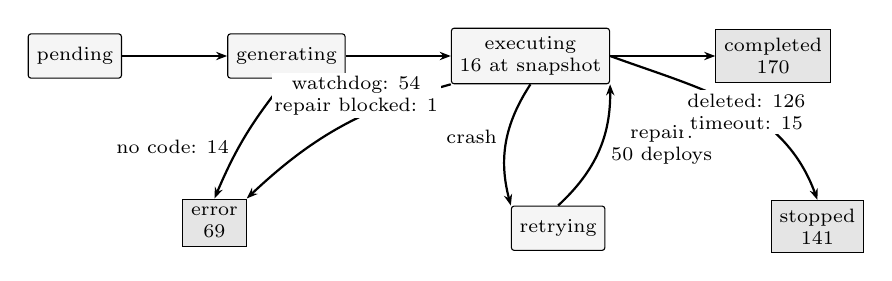
\begin{tikzpicture}[
  font=\scriptsize,
  svc/.style={draw, rounded corners=1pt, align=center, minimum height=16pt,
              inner sep=3pt, fill=gray!8},
  term/.style={draw, align=center, minimum height=16pt, inner sep=3pt,
               fill=gray!20},
  flow/.style={-{Stealth[length=4pt]}, thick},
  node distance=30pt and 38pt]

\node[svc] (pend) {pending};
\node[svc, right=of pend] (gen) {generating};
\node[svc, right=of gen] (exec) {executing\\16 at snapshot};
\node[term, right=of exec] (comp) {completed\\170};
\node[term] (err) at ($(gen.south) + (-26pt,-52pt)$) {error\\69};
\node[svc] (retry) at ($(exec.south) + (10pt,-52pt)$) {retrying};
\node[term] (stop) at ($(comp.south) + (16pt,-52pt)$) {stopped\\141};

\draw[flow] (pend) -- (gen);
\draw[flow] (gen) -- (exec);
\draw[flow] (exec) -- (comp);
\draw[flow] (gen.south) to[bend right=8]
  node[left, pos=.6]{no code: 14} (err.north);
\draw[flow] (exec.south west) to[bend right=14]
  node[above, pos=.42, align=center, fill=white, inner sep=1pt]
  {watchdog: 54\\repair blocked: 1} (err.north east);
\draw[flow] (exec.south) to[bend right=24]
  node[left, pos=.45]{crash} (retry.north west);
\draw[flow] (retry.north) to[bend right=24]
  node[right, pos=.55, align=center]{repair:\\50 deploys} (exec.south east);
\draw[flow] (exec.east) to[out=-20, in=110]
  node[fill=white, inner sep=1.5pt, pos=.55, align=center]
  {deleted: 126\\timeout: 15} (stop.north);
\end{tikzpicture}
}
\caption{Status machine with production counts ($n=\nWrappers{}$). The
crash-and-repair branch touched \nRetried{} wrappers across \nHealEvents{}
redeployments; most \texttt{error} outcomes are watchdog kills of long-cadence API
pollers, not faulty code (Section~\ref{sec:res-faults}).}
\label{fig:lifecycle}
\end{figure}

\subsection{Repair effectiveness and exposure}
\label{sec:res-heal}
\nRetried{} wrappers (\pctRetried\%; 26 spreadsheet, 14 API, 3 CSV) threw an
uncaught exception while running and received at least one repair, \nHealEvents{}
redeployments in all; a 44th crashed wrapper
never received a repair because the repair call itself hit the model quota, and
Section~\ref{sec:res-faults} counts it. Repair depth was \retryOnce{} wrappers at one
attempt, \retryTwice{} at two, and \retryThrice{} at three. ``Recovery'' can be read
three ways, which we keep apart and rank. The weakest
reading is recurrence: the same crash came back after the last repair for exactly one
of the 43, so 42 stayed crash-free. Final status is the next: \nRecovered{} of 43
(\pctRecovered\%) closed in a non-error state, a count that still includes the one
wrapper that burned all three attempts and shows non-error only because its resource
was deleted afterwards, which we do not score as a win. The reading we adopt as
primary is resumed output: 32 of 43 sent data again after their last repair, 20{,}351
points in all, about an eighth of everything collected, though one test feed accounts
for 17{,}466 of them. Repairs were fast and untouched by a person: a median
\healLatencyMedian{}\,s from crash to redeployment (quartiles 24.2 and 50.8\,s, 90th percentile \healLatencyPninety{}\,s, longest \healLatencyMax{}\,s), up to 30\,s of
which is the detection cycle. The typical crash arrived 16.8\,s into a run, in the
fetch-and-parse stage.

Recurrence and resumed output are only as strong as the exposure behind them, so we
measured, for each repaired wrapper, the time from its last repair to its last
evidence of life (last log entry, emitted point, or stored segment; the snapshot
for the three still executing). The 29 repaired file wrappers run once and exit, so
their ``no recurrence'' means only that the repaired run completed. The 14 repaired API pollers are the real test: they were
observed for a median \expApiMedianDays{} days after repair (quartiles \expApiQone{}
and \expApiQthree{}, maximum \expMaxDays{}, 230 wrapper-days in all) and survived 14 platform relaunch events (13 service restarts and one boot loop,
below) on 10 dates without a crash. Nineteen of the 43 later had their resource
deleted, eight of them as the event that ended observation, so for those the recovery
is unverified.

Two features of the timeline qualify the counts. For the first 65 days no repair
loop was active (it first appears in the logs on 2026-03-19); 36 crashes of the same
exit class went unrepaired in that stretch, and once the loop was on it repaired 24 of
those 36 wrappers, most in the mass relaunch below. And 31 of the 50 repair events land on a single day, when a credential fix set off a
redeploy that restarted every wrapper together, hours after a service boot loop had
cycled 623 times in 3.4 hours and respawned about 40 pollers per cycle (20{,}849
starts, recorded only by the wrappers' own log entries), so the events are correlated
rather than 50 independent failures;
restricted to each wrapper's first repair, the 17 that first crashed on other days
have a median 34.0\,s (range 15.5--80.4) against 33.2\,s for the 26-wrapper batch,
and 15 of those 17 ended non-error. Because each relaunch overwrites stderr, a triggering trace
survives only where the last run also crashed; for recovered wrappers we read the
cause from the fixes their code carries, so these counts describe the model's
\emph{repairs}, not independently observed causes.

\subsection{Faults inside and outside the manager}
\label{sec:res-faults}
% Failure root causes and self-healing outcomes (auto-generated from production dump).
% Requires \usepackage{booktabs}. \input this file into the IEEEtran document.
\begin{table}[t]
\centering
\caption{Why the 69 \texttt{error}-status wrappers ended there, and how the
repair loop fared over the 43 crashed wrappers and their 50 automatic repairs.}
\label{tab:errors}
\begin{tabular}{@{}llr@{}}
\toprule
\multicolumn{3}{@{}l}{\textbf{(a) Root causes of \texttt{error} status} ($n=69$)} \\
\midrule
Stage & Root cause & $n$ \\
\midrule
Generation & Model free-tier request quota (HTTP 429)\textsuperscript{c} & 10 \\
Generation & Model provider overloaded (HTTP 503) & 1 \\
Generation & Service restart during generation & 3 \\
Runtime & Execution watchdog (3600\,s), API pollers\textsuperscript{a} & 54 \\
Runtime & Crash; repair blocked by model quota (429) & 1 \\
\midrule
 & Total & 69 \\
\midrule
\multicolumn{3}{@{}l}{\textbf{(b) Repair outcomes} (43 repaired wrappers, all crashes exit~1)} \\
\midrule
\multicolumn{2}{@{}l}{Repaired once, crash never recurred} & 37 \\
\multicolumn{2}{@{}l}{Repaired twice, crash never recurred} & 5 \\
\multicolumn{2}{@{}l}{Still crashing after 3 repairs (retries exhausted)} & 1 \\
\midrule
\multicolumn{2}{@{}l}{Final status: completed / stopped / executing} & 28 / 8 / 3 \\
\multicolumn{2}{@{}l}{Final status: error (later watchdog timeout)\textsuperscript{b}} & 4 \\
\midrule
\multicolumn{2}{@{}l}{Crash-free after repair (recurrence)} & 42/43 \\
\multicolumn{2}{@{}l}{Median crash-to-redeploy repair latency} & 33.4\,s \\
\bottomrule
\multicolumn{3}{@{}p{0.95\columnwidth}@{}}{\footnotesize \textsuperscript{a}Marked by the watchdog's termination message; stderr held no traceback (53 of 54 blank, one harmless warning). See Section~\ref{sec:res-faults} for their coverage cost. \textsuperscript{b}Each of the four was repaired and never crashed again; the later \texttt{error} comes from the watchdog limit, not the repaired code. \textsuperscript{c}Another 51 generation failures (46 quota, 3 overload, 1 restart, 1 unrecorded) were deleted by their users and appear as \texttt{stopped}.} \\
\end{tabular}
\end{table}

This is the paper's central result, and it has two halves. Uncaught exceptions were
not rare: at least 56 wrappers, one in seven, exited with one at some point (the
count is a lower bound, since regeneration erases a wrapper's earlier log); 44 of
these were code faults the loop could address (43 repaired, one quota-blocked) and 12
cleared on a later relaunch with no code change, so were transient. The loop stopped
the crash in 42 of the 43 it reached, so nearly every wrapper that ended in
\texttt{error} did so for an operational reason. Table~\ref{tab:errors} sorts the
\nErrorW{} wrappers in \texttt{error} by cause, and one of them indicts the generated
code. Fourteen never reached the running stage: ten ran into the model's free-tier
request quota, one a provider overload, and three were cut off mid-generation when a
service restarted. The same status filter hides 51 more: every one of the 65 wrappers
without stored code is a generation failure (56 on quota, 4 on overload or restart,
1 unrecorded), and 51 of them were deleted by their users before the snapshot, so 16\%
of everything registered never got as far as running code. The larger set of 54 are API pollers the
3600\,s watchdog stopped between polling cycles, 53 of them leaving no traceback. These are
configuration faults of our own making, a platform timeout shorter than the feeds'
daily or monthly rhythm, marked by the watchdog's termination message and an empty
stderr. Fifteen more pollers were killed the same
way and later deleted by their users, so they appear as \texttt{stopped}
(Fig.~\ref{fig:lifecycle}); 69 of 184 API wrappers (38\%) were killed in all, 64 of
them one hour after the deploy that introduced the timeout, in the first monitor tick
past the limit, and they had shipped 61{,}627 points, 78\% of all API points. Read
from the generated code rather than the user's label, 34 of the 69 polled daily, 3
monthly, 26 yearly or slower, and 6 hourly-or-faster pollers were killed while idle
past the hour: while the limit was in force, no long-cadence API feed survived its
first idle hour. No kill is recorded after 2026-05-21, and the 16 pollers running at
the snapshot had been up for eight hours, so the limit was evidently relaxed late in
the run; the code at the pinned commit still defaults to 3600\,s. A third
operational class hides under \texttt{completed}: the operator's re-execute route
marks an API wrapper completed at launch, and the supervisor does not respawn
completed wrappers after a restart, so all 52 API wrappers in that state (24 daily, 27
yearly or slower) ended silently on a later deploy; none finished on its own. One wrapper
crashed and could not be mended because the repair call itself struck the quota
ceiling, the lone error-status case where generated code went unrepaired. Code
defects happen at the rate generation makes them and the loop retires them at machine
speed; what is left on the operator's desk is the envelope of quota, credentials,
service availability, and cadence-to-timeout matching. The specific watchdog and
quota are this deployment's instantiation; the category is what we expect to
transfer, and the manager removes the per-source \emph{code}, not every per-source
decision.

\subsection{Repair case studies}
\label{sec:res-cases}
Four wrappers, chosen to exercise the boundary rather than sampled at random,
illustrate the partition. A yearly urban-waste API wrapper crashed 82\,s into its
backfill on a timezone-aware-versus-naive comparison; the repair normalizes both
bounds and downgrades an empty fetch to a log line (34.7\,s, 596 points). An
air-quality wrapper whose URL already pinned a date window had a second one appended
and got an HTTP~400; the repair strips the duplicate and swallows any residual 400
(51.3\,s, 395 points, still streaming). A workbook repeated its localized year header
among the values, so the wrapper died converting it to an integer; the repair coerces
to numeric and drops non-numeric rows, as do three siblings (61.6\,s). The
out-of-scope case is a single-column export: three repairs tried delimiter tricks but
could not invent a $(\textrm{time},\textrm{value})$ pair, while a two-column sibling
was repaired at once. Two of the four ``recover'' by absorbing an upstream error rather than extracting
the intended data, which is exactly the move that can mask data loss behind a clean
exit; both follow a rule in our own generation prompt (never raise on an HTTP error,
return an empty batch), so the masking is policy we wrote. The manager mends code;
it cannot supply data the source withholds. Pre-repair code is not retained, so the masking rate cannot be
measured by diff; a static scan of the final code of the 43 repaired wrappers against
the 288 never-repaired ones with code finds the swallow-and-continue and coercion
patterns equally common in both (they come from the template), with one exception: a
bare \texttt{except} clause appears in six repaired wrappers (seven clauses) and in
none of the controls.

\subsection{Cost, and a consistency check on values}
\label{sec:res-cost}
The platform logged no token counts and ran on the provider's free tier, so model
spend was zero and the binding limit was a daily request quota rather than money;
what the run would have cost at paid rates is an estimate we label as such. From the prompt templates at the deployed commit and the 331 wrappers with stored
code we measured the fixed prompt (\costFixedApiTok{} tokens for an API source, about
3{,}200--3{,}300 for files, at four characters per token), the variable sample and
metadata, and the generated code (median \costCodeTok{} output tokens), priced at the
rates published on \costPriceDate{} for the model the alias resolved to
(\costInPrice{} and \costOutPrice{} USD per million input and output tokens). A generation then costs about \costGenMedianUSD{} USD at the median and a
repair, which carries the crashed source and its trace, about \costRepairMedianUSD{}
USD; the \nWrappers{} generation attempts and \nHealEvents{} repairs together fall
between \costTotalLowUSD{} USD with no tool calls and \costTotalHighUSD{} USD if every
API wrapper spent its full budget of probing calls, about three times that at the
successor model's rates, plus whatever unlogged reasoning tokens added. The estimate omits the corrective prompt a failed static check earns, prices the last
fifteen days at the earlier model's rate, and treats probing calls as flat context; no
hand-written wrapper exists for comparison. The whole run would have cost 1.6 to 7.4
cents per data-yielding wrapper at paid rates, so the 57 quota faults, 14\% of
everything registered, were avoidable for less than an engineer-hour.

The collector checks shape, not whether values match the source, and the snapshot
retains no copy of the sources, so value correctness could not be verified from the
dump. As a bounded substitute we took the stored code of
\spotN{} API wrappers whose endpoints are public and need no credential (seven from
a national statistics portal, one weather feed; six of the eight had been
repaired), re-ran only their extraction logic against the live source three months
after the snapshot (at most three requests each), and compared the fresh
$(\textrm{timestamp},\textrm{value})$ pairs with the dumped points over the
overlapping range; the same code re-run against the same endpoint cannot reveal a
wrong column or unit, so this is a consistency check only. All \spotReachable{} sources were still reachable; six wrappers
yielded \spotOverlap{} overlapping timestamps (77 of them from the two never-repaired
wrappers, 18 from repaired code), of which \spotMatch{} matched exactly and
\spotMismatch{} differed, every difference an upstream revision of a published
statistic (one annual value revised by 0.2\%, ten monthly values revised down by up to
1.9\%), so none is an extraction error. Four wrappers matched on every
overlapping point; two were inconclusive (a deleted resource with no stored
segments, and a request budget spent outside the stored range). This small
convenience sample leaves spreadsheets, where 26 of the 43 crashes occurred,
unchecked.

\subsection{Pipeline integrity}
\label{sec:res-pipeline}
Of the \nDataPoints{} points emitted, 148{,}131 reach the resource store and
84{,}431 survive consolidation and merging; the attrition is bookkeeping (deleted
resources, regeneration, deduplication), not loss. Over 30 days the collector rejected
nothing on schema grounds, all 153 control-plane messages in an 8.3-hour window
arrived, and a container rebuild restarted all 16 running wrappers, 15 of which
resumed from their watermarks.

\section{Lessons and Threats to Validity}
\label{sec:discussion}

\subsection{Lessons for operators}
Each of these cost us data or the means to audit it; each is a rule the platform
could enforce. (1) Derive the execution timeout from the generated polling period, or
make the watchdog idle-aware: a fixed 3600\,s limit killed every daily, monthly, and
yearly API poller within a tick of its first idle hour, 64 on the day it shipped.
(2) Alert on clean exits that emit nothing and on pollers that stop being respawned:
22 wrappers completed with zero points and 52 API pollers were orphaned by a
bookkeeping status, both indistinguishable from a healthy run. (3) Budget the model
quota as a dependency: it stopped 57 wrappers, 14\% of everything registered, for
want of a few dollars. (4) Retain stderr and the source sample across relaunches: the
relaunch overwrote the trace for 42 of the 43 repaired wrappers and no source copy
exists, so neither cause nor value can be audited. (5) Pin the model version: the
alias resolved to two models during the run. (6) Monitor values, not exits: repair can
mask data loss behind a clean status. (7) Guard the supervisor against restart storms:
the boot loop of Section~\ref{sec:res-heal} silently killed its children 623 times in
an afternoon, recorded only in the wrappers' start entries.


\subsection{Threats to validity}
\emph{Internal.} The evidence is observational, from one deployment with no control
arm; the pre-automation period is a reference, the crash events are correlated, and for
repaired wrappers the cause is read from the fix because the relaunch destroyed the
trace. The authors assigned root causes from logs without a second rater.
\emph{Construct.} Recovery is scored as resumed output, backed by the exposure
analysis; the collector inspects shape, never truth; the re-extraction check covers
only public, stable sources, mostly through unrepaired code; the cost figure is a
counterfactual estimate. \emph{External.} One model family, one region, a
user-selected source mix, and a rule list that accreted over the run, so the
code-defect rate is partly co-produced by curation; the alias resolved to one model
until 2026-05-20 and to its successor by 2026-05-27, so the numbers pool two models.
We do not ablate probing, the template, or whole-file repair. \emph{Security.}
Model-written code runs as live processes contained only by process isolation, a
semaphore, and the watchdog, and the generation prompt ingests a live source sample,
so an injected instruction in a CSV or API reply could steer code running with the
resource's credentials; the static check catches unfilled placeholders, not intent.
An egress allow-list and a filesystem-free sandbox are the mitigations we would add.

\section{Conclusion}
\label{sec:conclusion}

We operated LLM-generated extraction wrappers as live infrastructure for
\deploymentDays{} days: \nWrappers{} wrappers, \nDataPoints{} points, at least one
wrapper in seven crashing, the repair loop stopping the crash in 42 of the 43 it
reached and restoring output in 32 at a median \healLatencyMedian{}\,s. The faults
that filled the error column were operational: a timeout we set, a quota we exhausted,
a service we restarted. What stayed unresolved was smaller and harder: 22 clean exits
with nothing, 52 pollers orphaned by a status, one crash the loop could not mend, one
it never reached. The agenda follows: check extracted values for meaning, and fold
cadence, quota, and credential faults into the manager as state it owns.

% \balance left out: with the references spilling to a second page it strands one entry on a third.
\section*{Acknowledgment}
This research was funded by the PRR -- Plano de Recupera\c{c}\~ao e Resili\^encia
and by the NextGenerationEU funds at Universidade de Aveiro, through the scope of
the Agenda for Business Innovation ``ATT -- Agenda Mobilizadora Acelerar e
Transformar o Turismo'' (Project no.\ 47 with the application C645192610-00000060).

% Mandatory funder logo bar, used as supplied (composed bar, colour variant); do
% not recompose or crop it. Set inline so it stays with the funding statement.
\par\vspace{3pt}
\noindent
\includegraphics[width=\columnwidth]{figures/BARRA_LOGOS-COR.png}

\bibliographystyle{IEEEtran}
\bibliography{refs}

\end{document}
